

        \begin{frame}{Starting point}
        \begin{figure}[b]
        \begin{minipage}{0.12\textwidth} 
        \changeurlcolor{mNormal} \qrcode[height=1.2cm]{https://arxiv.org/abs/1701.09137}   
        \end{minipage} 
        \hfill 
        \begin{minipage}{0.85\textwidth} 
        \raggedright
        \emph{Airy structures and symplectic geometry of  topological recursion}, M. Kontsevich and  Y. Soibelman, 2017, {\color{pink}{\tt arXiv:1701.09137}} [math.AG]
        \end{minipage}
        \end{figure} 
        \end{frame}
    
        %\begin{frame}{Possible things to take away}
        %Hopefully, some knowledge of deformation quantisation.
        
        %The definition of an Airy structure.
        %\end{frame}
    
    
        \begin{frame}{Deformations}
        A formal deformation replaces a \( \mathbf{k} \)-algebra \((A,\cdot)\), with a non commutative \(\mathbf{k} \lBrack \hslash \rBrack \)-algebra \( (A_{\hslash},\star)\), such that
        \[ 0 \rightarrow \hslash A_{\hslash} \rightarrow A_{\hslash} \rightarrow A \rightarrow 0, \]
        eg \( A_{\hslash}/\hslash A_{\hslash} = A\).
        
        Gives a deformed product: \( a_{\hslash} \star b_{\hslash} = a \cdot b + O(\hslash)\).
        
        \emph{Deformation quantisation} is formal deformation with extra constraint. \(A\) is Poisson algebra, Poisson bracket \( \{ \cdot, \cdot\}\): 
        \[ a \star b - b \star a = \hslash \{ a, b\} + O(\hslash^2)\] 
        matches Poisson structure.
        
        \end{frame}    
            
        \begin{frame}
        \begin{ex}[Weyl algebra]
        Replacing the ring of functions \( \mathbf{k}[x,y]\), (with Poisson bracket \(\{ x,y\}=1)\), with a ring of operators \( \mathbf{k}[x,\hslash \frac{\partial}{\partial x} ]\lBrack \hslash \rBrack \) is a (representation of a) deformation quantisation.
        \end{ex} 
        
        Need a space on which these operators act -- wavefunctions.

        \end{frame}
        
        
        \begin{frame}{The big picture}
        Symplectic affine symplectic space \((W_\Sigma, \mathcal{O}(W_\Sigma))\).

        \begin{center}
        \begin{tikzpicture}[
            node distance=2cm and 3cm,
            ar/.style={->,>=latex},
            mynode/.style={
              draw,
              text width=3cm,
              minimum height=1cm,
              text centered
              }
            ]
            
            \node[mynode] (ar) {Airy structure\\ on \(\mathcal{O}(W_\Sigma\))};

            
            \node[mynode, right=of ar] (ls) {Lagrangian subvariety \( \mathcal{O}(\mathbb{L})\) };

            \node[mynode,below=of ar] (Asig) {A tensor \(A_\Sigma \cong \omega_{0,3}\)};

            
            \node[mynode,below=of ls] (tr) {Topological recursion \( \omega_{g,n}\)};

            \draw[ar] 
              (ls) -- node[right] {\parbox{3cm}{Deformation Quantisation}} (tr);
            \draw[ar] 
              (ar) -- node[above] {Encodes} (ls);
            \draw[ar] 
              (ar) -- node[above] {} (Asig);
            \draw[ar] 
              (Asig) -- node[above] {Initial data for} (tr);

        \end{tikzpicture}
        \[ 0 \rightarrow \mathcal{J} \rightarrow  \mathcal{O}(W_\Sigma) \rightarrow \mathcal{O}(\mathbb{L}) \rightarrow 0 \]
        \end{center}
        
        \( \omega_{g,n} \) meromorphic poly-differential.
        
    
        % linear symplectic vector space 
        % lagrangian subspaces
        % non degenerate (2,0) form \(\omega\)
        % quadratic 
        
        
        % coefficients of variety - tensors
        % coefficients turns out to be tensors
        % remind that describing geometry of subvariety
        % pictures are encoding lagrangian
        
        %lagrangian subvariety - tensors
        
        
        % history - quadratic lagrangian - quantisation understood - arise in givental, varieties
        
        % get lie algebra -> can quantise lie algebra
        % hamiltonians symplectic group
    \end{frame}
    
    \begin{frame}{What we added}
         Need \emph{deformation quantisation}, \( \mathcal{O}(W_\Sigma) \lBrack \hslash \rBrack \).
    
        This gives an understanding  of \emph{reduction} of {wavefunctions}, \( \psi_{\mathbb{L}}  \rightarrow \psi_{\mathcal{B}}\).
        
        \[ \psi_{\mathbb{L}} \in \text{Hom}\left( \widehat{\mathcal{O}}(W_\Sigma)\lBrack \hslash \rBrack / ( \mathcal{J} ) , \widehat{\mathcal{O}}(W_\Sigma)\lBrack \hslash \rBrack \right), \]
        
        Connection between \(A_\Sigma\) and the  \emph{Donagi Markman cubic}, which is a cohomology class: \([A_\Sigma]\)
    \[ a_{ijk} x^i x^j x^k  = S_{0,3} \cong A_\Sigma =  a_{ijk} x^i \otimes x^j \otimes x^k, \]

    \end{frame}

    \begin{frame} 
    \( \psi_{\mathbb{L}}\) produced by deformation quantisation. Wavefunctions are a generating function:
    \[ \psi_{\mathbb{L}} = \exp \left[ \frac{1}{\hslash} ( S_{0,3} +S_{0,4} + \dots ) + (  S_{1,1} + \dots ) + \hslash (  S_{2,1} + \dots ) \right], \]
    where \( S_{g,n} \cong \omega_{g,n}\). 
    
    \( \psi_{\mathcal{B}}\) depends on cohomology classes, 
    \[ \psi_{\mathcal{B}} = \exp \left[ \frac{1}{\hslash}\, \mathcal{S} \right] \]
    \( \mathcal{S}\) series in \(\hslash\) on \( \mathcal{B}\), \(\mathcal{B}\) moduli space of deformations of \(\Sigma\) in a surface.
    
    Quantisation of moduli space of deformations of curves?
    \end{frame}


    \begin{frame}{What else we added}
    
    Verified a formula for the reduction of wavefunctions following Kontsevich and Soibelman
    \begin{thm}
    \[ \psi_{\mathcal{B}} = \int D x\, \psi_{\mathbb{L}} \, \exp\left( \frac{1}{\hslash} Q(x^{\sbt}, z^{\sbt}) \right) \]
    \end{thm}
    \(Q\) determined from a fibre product. \(G \subset W_\Sigma\) coisotropic.
    \begin{center}
        \begin{tikzcd}[ampersand replacement=\&]
        \mathcal{O}_{W_\Sigma } \otimes_\mathbf{k}\mathcal{O}_{G }^{G^{\perp}}  \arrow[r] \arrow[d] \& \mathcal{O}_{G} \arrow[d]\\
        \mathcal{O}_{\mathbb{L}} \arrow[r] \&  \mathcal{O}_{G \cap {\mathbb{L}}}   \cong \mathcal{O}_{\mathcal{B}}
        \end{tikzcd}
    \end{center}
    \( \psi_{\mathcal{B}}\) associated to deformation quantisation of \( \mathcal{O}_{\mathcal{B}}\).
    \end{frame}
    
    
    \begin{frame}{Papers}
    \begin{figure}[t]
        \begin{minipage}{0.12\textwidth}    
        \changeurlcolor{mNormal}\qrcode[height=1.2cm]{https://arxiv.org/abs/2206.04848}
        \end{minipage} 
        \hfill
        \begin{minipage}{0.85\textwidth} 
        \raggedright
        \emph{Deformation quantisation of the conic and symplectic reduction of wavefunctions}, 
        M. Swaddle, 2022, {\color{pink}{\tt arXiv:2206.04848}} [math-ph] 
        \end{minipage}
    \end{figure}
    
    \begin{figure}[b]
        \begin{minipage}{0.12\textwidth}    
        \changeurlcolor{mNormal}\qrcode[height=1.2cm]{https://arxiv.org/abs/2012.00254} 
        \end{minipage} 
        \hfill 
        \begin{minipage}{0.85\textwidth}
        \raggedright
        \emph{Airy structures and deformations of curves in surfaces}, W. Chaimanowong, P. Norbury, M. Swaddle, and M. Tavakol, 2020, {\color{pink}{\tt 	arXiv:2012.00254}} [math.AG]
        \end{minipage}
        \end{figure}
    \end{frame}

    
    \begin{frame}{Outline}
    \tableofcontents
    \end{frame}

    \frame{\sectionpage}

    \begin{frame}{Formal completion of a ring}
    Complete at a maximal ideal \( \langle x \rangle \):
    \begin{ex} \[ \mathbf{k} \lBrack x \rBrack   = \lim_{n}  \frac{\mathbf{k}[x]}{\langle x \rangle^n} \]
    \end{ex}
    Limit is limit in category of rings, \( \mathbf{k}\lBrack x \rBrack \) is something all \( \mathbf{k}[x] / \langle x \rangle^n\) map into.
    
    More generally a terminal object \(R_I = \lim_n R/I^n\). 
    
    Actually think lazy evaluation, always think in terms of finite \(n\)-th quotient \(R/I^n\), and can always go to to \(n+1\) if needed.
    
    \begin{defn}\( \Spec( R/I^n)\) called the \(n\)-th formal neighbourhood.
    \end{defn} 
    \end{frame}
    
    \begin{frame}{Why is this important?}
    In the application to topological recursion, \( \mathbb{L}\) is only topologically a point in an infinite dimensional symplectic space \(W_\Sigma\). However, the formal neighbourhoods of \( \mathbb{L}\) contain rich information.
    \end{frame}
    
    
    
    % say more completion
    
    % defn of completion
    
    % why need completions
    % forced to do power series
    
    % L topologically a point in W 
    % look in formal neighbourhoods of point
    % model example something infinite dimensions, 
    % in that case underlying thing topologically a point
    % look in formal neighbourhoods
    % extract interesting information (tr etc)
    
    
    % example Lagrangian
    % symplectic affine spaces
    
    % add lagrangian closed poisson bracket
    
    % more definitions
    
    \begin{frame}{The conic}
    An important example to take away.
    
     \( \mathbf{k}\) field characteristic zero.
    
    \vspace{1em}
    \begin{ex}[Conic in the plane]
    Consider \( \mathbf{k}[x,y]\) as Poisson algebra, Poisson bracket \( \{y,x\}=1\).
    
    Example Lagrangian:
    \[\mathbb{L} = \Spec \left( \frac{\mathbf{k}[x,y]} {  \mathcal{J}(\mathbb{L})} \right) \]
    where 
    \(  \mathcal{J}(\mathbb{L}) = \langle -y +  x^2 + 2 \,x\, y + y^2\rangle\)
    \end{ex} 
    Ideal must be closed under Poisson bracket: 
    \[ \{ \mathcal{J}, \mathcal{J} \}  \subseteq \mathcal{J} \]
    \end{frame} 
    %wait I guess I mean R/I , R/I = 
    
    % limit first, then completion
    

    
    
    \begin{frame} 
    \begin{figure}
    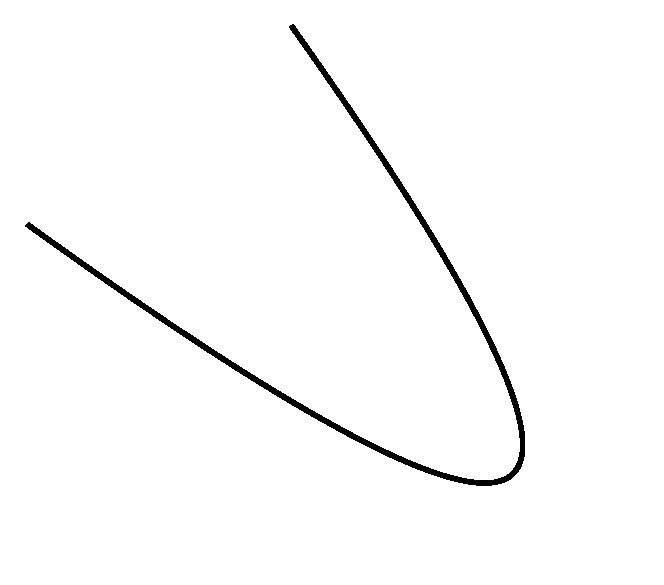
\includegraphics[width=4cm]{sections/out.pdf}
    \caption{\(-y+x^2+2 xy+y^2=0\)}
    \end{figure}    
    \end{frame} 
    
    \begin{frame}
    Solve \(-y + x^2 + 2\, x\, y + y^2 = 0\) for \(y(x)=u_0(x)\) via fixed point iteration. 
    
    Algebraically: completion at maximal ideal \( \langle x, y \rangle \):
    \[ \widehat{\mathbb{L}} = \mathrm{Spf} \left( \mathbf{k}[\![x,y ]\!]/ \langle y - u_0 \rangle \right) \]
    Formal series
    \[ u_0 = x^2 + 2 x^3 + 5 x^4 + \dots \]
    Encodes the \emph{Catalan numbers}:
    \[ \{1,2,5,14,\dots \}\]
    Formal series can contain interesting data. 
    \end{frame}
    
    \begin{frame}{Fixed point iteration}
        Finding the formal series.
        
        Initial condition \(y^{[0]} = 0\).
        \begin{align*} 
        y^{[n]} &= x^2 + 2 \,x\, y^{[n-1]} + y^{[n-1]}\, y^{[n-1]} \\
        y^{[1]} &= x^2 \\
        y^{[2]} &= x^2 + 2 \, x^3 + (x^2)\, (x^2) 
        \end{align*}
        Coefficients stabilise and \(y^{[n]} \rightarrow u_0(x)\). This idea generalises to the infinite dimensional case.
    \end{frame}
    
    
    \begin{frame}{Trees}
    Catalan numbers count rooted binary trees (notion of left/right)
    \begin{center}
    \begin{tabular}{c c c } 
    
    \tikz [tree layout, baseline=(x0.base), grow'=up, significant sep=1em, sibling distance=7mm, level distance=7mm]
     \graph {
        [nodes={circle, draw, inner sep=0pt, minimum size=2mm, as =}]{ x0};
        // [nodes={circle, inner sep=0pt, minimum size=2mm, fill, as=}]{ x0 -- x1 };
        // [nodes={circle, fill={pink} }]{ x1 -- {x2,x3}};
    };  
    
    &
    \tikz [ baseline=(a.base), tree layout, significant sep=1em, grow'=up, sibling distance=7mm, level distance=7mm]
    \graph {
        [nodes={circle, draw, inner sep=0pt, minimum size=2mm, as =}]{ a};
        // [nodes={circle, inner sep=0pt, minimum size=2mm, fill, as=}]{a -- {b--{c}} };
        // [nodes={circle, fill={pink} }]{b-- d};
        // [nodes={circle, fill={pink} }]{c --{e,f}};
        };
    & 
    
    \tikz [ baseline=(a.base), tree layout, significant sep=1em, grow'=up, sibling distance=7mm, level distance=7mm]
    \graph {
        [nodes={circle, draw, inner sep=0pt, minimum size=2mm, as =}]{ a };
        // [nodes={circle, inner sep=0pt, minimum size=2mm, fill, as=}]{ a -- { b-- {c,d}} };
        // [nodes={circle, fill={pink} }]{ c -- {e,f}};
        // [nodes={circle, fill={pink} }]{ d -- {g,h}};
        };
    
    \tikz [ baseline=(a.base), binary tree layout, significant sep=1em, grow'=up, sibling distance=7mm, level distance=7mm]
    \graph {
        [nodes={circle, draw, inner sep=0pt, minimum size=2mm, as =}]{ a };
        // [nodes={circle, inner sep=0pt, minimum size=2mm, fill, as=}]{ a -- b -- { d -- {e }} };
        // [nodes={circle, fill={pink} }]{ b -- c};
        // [nodes={circle, fill={pink} }]{ d -- f};
        // [nodes={circle, fill={pink} }]{ e -- {g,h}};
        };
    \\
    & &  \\ 
    \(x^2\) & \( 2 x^3\) &  \( 5 x^4 \)
    \end{tabular}
    \end{center}
    Drawn up to \( \cong\).
    \[ u_0(x) = x^2 + 2 x^3 + 5 x^4 + \dots \]
    \end{frame}
    
    
    \begin{frame}{Preview: Airy structures}
    Going to be a weighting with coefficients \( ( a , b , c )\)
    \[ \mathbf{k}[x,y] / \langle-y + {\color{pink} a}\, x^2 + 2 \,  {\color{pink} b} \,x\, y +  {\color{pink} c}\, y^2\rangle \]
    This will put a label/weighting on nodes in the tree.
    \[ u_0 = ({\color{pink} a})\, x^2 + ({\color{pink} 2\, b\, a} )\,x^2 + ({\color{pink} 4 \, b^2\, a + c \, a^2 } ) x^4 + \dots \]
    \end{frame}
    
    
    
    \begin{frame}{Preview}
    We will generalise this example following Kontsevich and Soibelman to arbitrary (and infinite) dimensions.
    \[ x\rightarrow \{x^1,x^2, \dots \}, y \rightarrow \{y_1, y_2 \dots\}\] 
    Quadratic replaced by a collection of polynomials \(H_i\).
    \[ H_i = -y_i + a_{ijk}x^j x^k + 2 b_{ij}^k x^j y_k + c_{i}^{jk} y_{j} y_k\]
    Scalar coefficients become tensors \(a \rightarrow a_{ijk}\).

    Coefficients in series \(u_{0}(x) \rightarrow u_{0,i}(x^{\sbt})\) become contraction of tensors, eg: 
    \[u_{0,i} = a_{ijk} x^j x^k + 2 b_{ij}^k a_{k st}x^j x^s x^t + \dots \]
    
    
    
    \end{frame}

    \begin{frame}{Finiteness}
    A key component is the choice of topology.
    
    Need to ensure sums converge or there is finiteness.
    
    Need to ensure contraction of tensors is finite, eg:
    \[ 2 b_{ij}^k a_{k st}\]
    
    

    %Pair a finite list and an infinite list
    %\[ \texttt{sum} \quad \$ \quad  \texttt{zipWith} \quad (*) \quad [1,2,\dots,N] \quad [1,2,\dots]\]
    \end{frame}

    
    %  x2 --[bend right=20] x4 , 
    % x2--[bend left=20] x4 , 
    
    
    % \quad 
